\documentclass[../DoAn.tex]{subfiles}
\begin{document}
% Chương này có độ dài từ 9 đến 11 trang.

% \textbf{Lưu ý}: Mỗi chương nên có thêm 1 đoạn mở đầu chương và kết thúc chương, mở đầu giới thiệu những nội dung sẽ trình bày trong chương, kết thúc tổng kết lại các nội dung đã trình bày

\section{Khảo sát hiện trạng}
\label{section:2.1}
Trong thời đại hiện nay, thương mại điện tử đang dần trở thành một lĩnh vực không thể thiếu trong đời sống, không chỉ đối với các mặt hàng như thời trang, thực phẩm. Việc khảo sát các hê thống thương mại điện tử về sách hiện đang tồn tại giúp chúng ta hiểu rõ hơn về sự phát triển và đa dạng của ngành này. Dưới đây là một cái nhìn tổng quan về các hệ thống phổ biến và đang được sử dụng rộng rãi:

\textbf{Fahasa.com:} Fahasa.com là website thương mại điện tử chính thức của tập đoàn Fahasa, một trong những nhà sách lớn nhất Việt Nam. Kể từ khi ra mắt vào năm 2012, Fahasa.com đã trở thành một trong những điểm đến trực tuyến uy tín và phổ biến nhất dành cho những ai yêu thích sách và tri thức.

Trang web cung cấp hàng trăm nghìn đầu sách thuộc nhiều chủ đề như giáo trình, văn học, kinh tế, kỹ năng sống và hàng ngàn sản phẩm văn phòng phẩm, đồ chơi trí tuệ cùng với các dịch vụ in ấn, photo và laminat. Khách hàng có thể dễ dàng tìm kiếm, đặt mua và nhận sản phẩm tại nhà thông qua các dịch vụ giao hàng hiệu quả của Fahasa.com. ngoài ra trang web còn kết hợp với các chi nhánh cửa hàng thực tế của Fahasa để đạt hiệu quả cáo trong việc bán hàng. 

\textbf{Vinabook.com:} VinaBook.com là một trong những website thương mại điện tử hàng đầu Việt Nam trong lĩnh vực bán sách và văn hóa đọc. Ra đời vào năm 2009, VinaBook.com đã trở thành điểm đến quen thuộc của hàng triệu độc giả và người yêu sách trên cả nước.

Trang web cung cấp một danh mục sách phong phú, bao gồm hàng trăm nghìn đầu sách thuộc các thể loại như giáo trình, tham khảo, văn học, kinh tế, kỹ năng sống và nhiều lĩnh vực tri thức khác. Ngoài sách, VinaBook.com còn cung cấp các sản phẩm văn phòng phẩm, đồ chơi trí tuệ và các dịch vụ in ấn, photo, laminat... Khách hàng có thể dễ dàng tìm kiếm, lựa chọn và đặt mua sản phẩm một cách nhanh chóng với các chính sách giao hàng và thanh toán linh hoạt.

Bên cạnh đó, VinaBook.com còn cung cấp nhiều nội dung hữu ích như tin tức, bài viết, đánh giá sách, giới thiệu tác giả nhằm mang đến cho người dùng những trải nghiệm mua sắm và tìm hiểu tri thức thú vị. Với giao diện thân thiện, dễ sử dụng và chính sách bán hàng minh bạch, VinaBook.com đã trở thành một trong những địa chỉ mua sắm sách và văn hóa đọc uy tín và phổ biến nhất tại Việt Nam.

Dựa trên phân tích trên, mỗi hệ thống có các ưu và nhược điểm riêng. Để phát triển một hệ thống thương mại điện tử  hiệu quả, tôi sẽ kết hợp các tính năng tốt nhất từ các hệ thống hiện có và tối ưu hóa chúng để đáp ứng nhu cầu và mong đợi của người dùng.

Các tính năng phần mềm quan trọng cần phát triển sẽ bao gồm:
\begin{itemize}
    \item \textbf{Tính năng học trực tuyến đa dạng:} Tạo ra một loạt các tính năng học trực tuyến như video học, tài liệu tương tác, bài tập , và hệ thống đánh giá để cung cấp cho người dùng trải nghiệm học tập đa dạng và phong phú.
    \item \textbf{Tính năng đặt hàng và thanh toán trực tuyến:} Phát triển tính năng đặt hàng trực tuyến, giúp khách hàng tiết kiệm thời gian, dễ dàng so sánh giá với các trang thương mại điện tử khác
    \item \textbf{Tính năng khiếu nại:} Xây dựng tính năng gửi phản hồi từ khách hàng giúp cải thiện chất lượng dịch vụ của nhà sách cũng như bên vận chuyển.
    \item \textbf{Hệ thống quản lý:} Tạo ra hệ thống quản lý đơn giản giúp nhà sách có thể quản lý được các đầu sách, đơn hàng.
\end{itemize}
Những tính năng này sẽ được phát triển và tối ưu hóa để tạo ra một hệ thống thương mại điện tử phù hợp với các nhà sách có quy mô vừa và nhỏ, linh hoạt và tiện ích, đồng thời đảm bảo rằng nó đáp ứng được các yêu cầu và mong đợi của cả người dùng và nhà quản lý.

\section{Tổng quan chức năng}
\label{section:2.2}

\label{subsection:2.2.1}

Hệ thống bao gồm các tác nhân sau:

\textbf{Admin}: Có quyền cao nhất trong hệ thống và có thể quản lý toàn bộ thông tin và hoạt động của người dùng. Quản lý các thông tin vê đơn hàng, sách, danh mục sách, khiếu nại từ người dùng.

\textbf{Người dùng}: Đăng nhập. xem sách, tìm kiếm sách theo thể loại, đầu mục. Thêm sách vào giỏ hàng và đặt đơn hàng, thanh toán online.

\textbf{Khách}: Đăng kí tài khoản, xem sách, tìm kiếm sách theo đầu mục, tên.

\begin{figure}[H] % Chèn hình ảnh vào vị trí chính xác
\centering
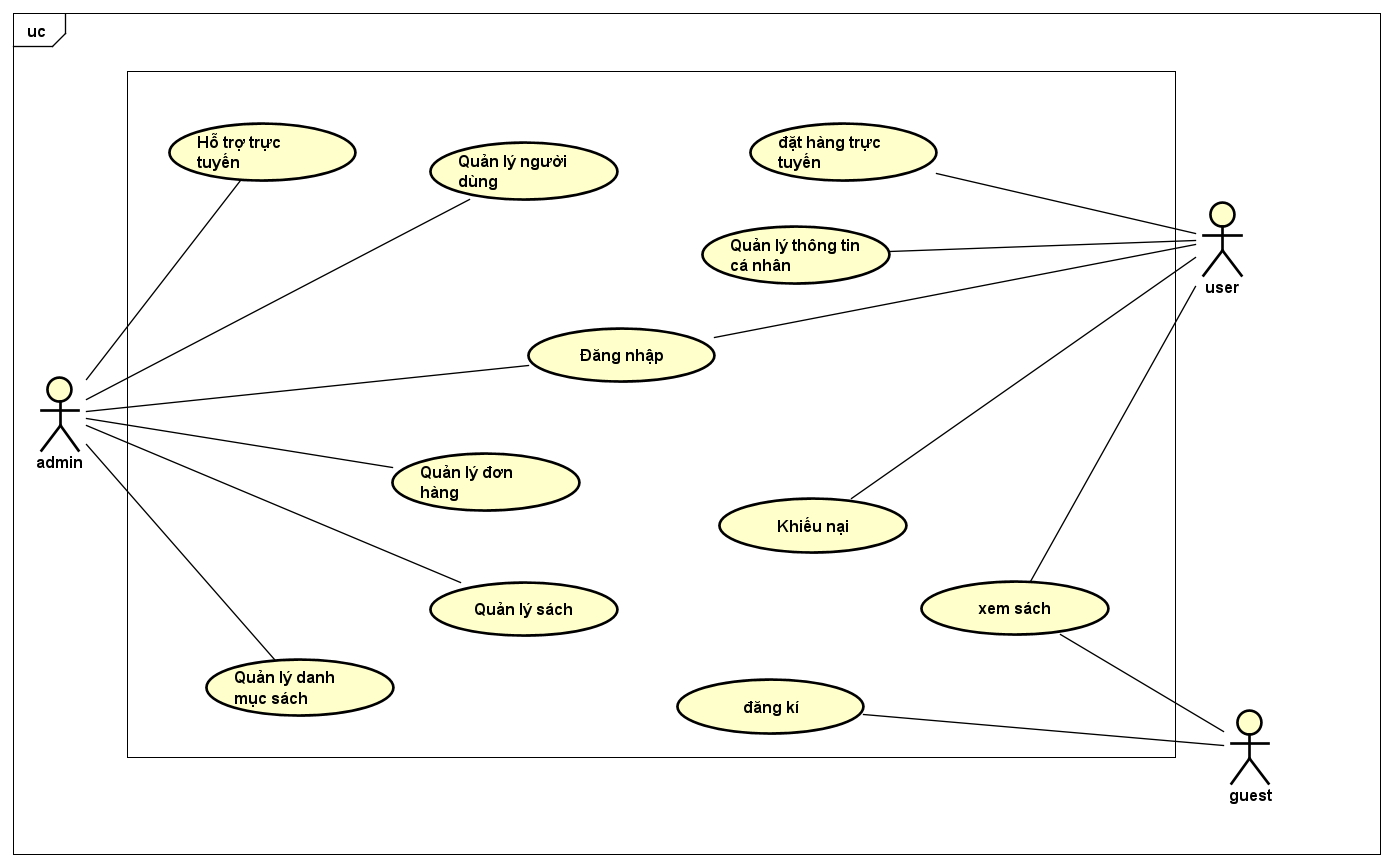
\includegraphics[width=1\linewidth]{Hinhve/thiết kế tổng quát.png}
\caption{Sơ đồ use case tổng quan hệ thống}
\label{fig:UsecaseOverview}
\end{figure}


\subsection{Biểu đồ use case phân rã use case "Đặt hàng trực tuyến"}
\label{subsection:2.2.2}
% Với mỗi use case mức cao trong biểu đồ use case tổng quan, sinh viên tạo một mục riêng như mục \ref{subsection:2.2.2} và tiến hành phân rã use case đó. Lưu ý tên use case cần phân rã trong biểu đồ use case tổng quan phải khớp với tên đề mục.

% Trong mỗi mục như vậy, sinh viên vẽ và giải thích ngắn gọn các use case phân rã.
\begin{figure}[H] % Chèn hình ảnh vào vị trí chính xác
\centering
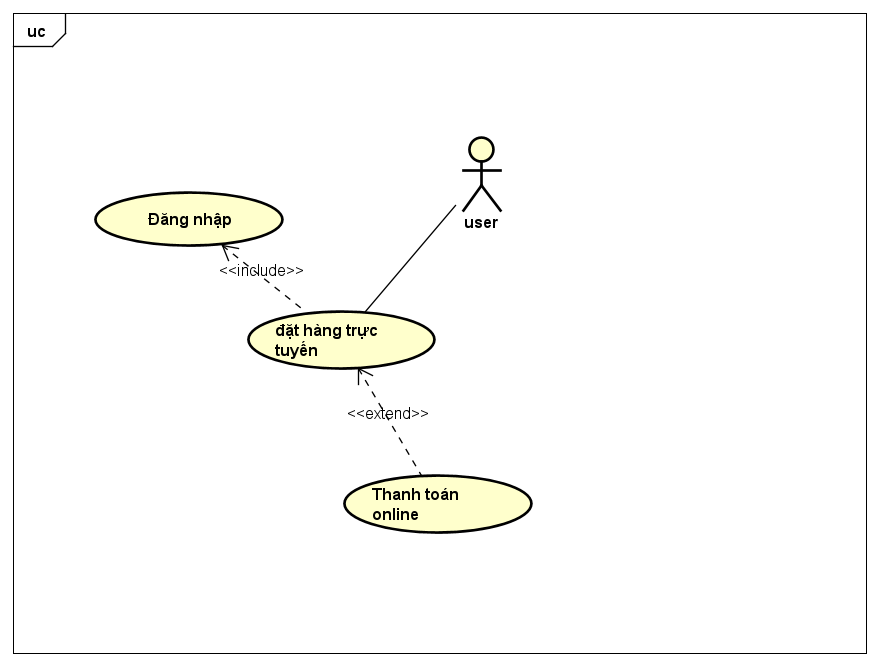
\includegraphics[width=1\linewidth]{Hinhve/Đạt hàng trực tuyến.png}
\caption{Sơ đồ use case "Đặt hàng trực tuyến"}
\label{fig:UsecaseOrderOnline}
\end{figure}
Với use case này cho phép người dùng đã có tài khoản có thể đăng nhập, chọn các sản phẩm vào giỏ hàng và đặt hàng trực tuyến tại trang web.

\subsection{Biểu đồ use case phân rã use case "Quản lý danh mục sách"}
\label{subsection:2.2.3}
\begin{figure}[H] % Chèn hình ảnh vào vị trí chính xác
\centering
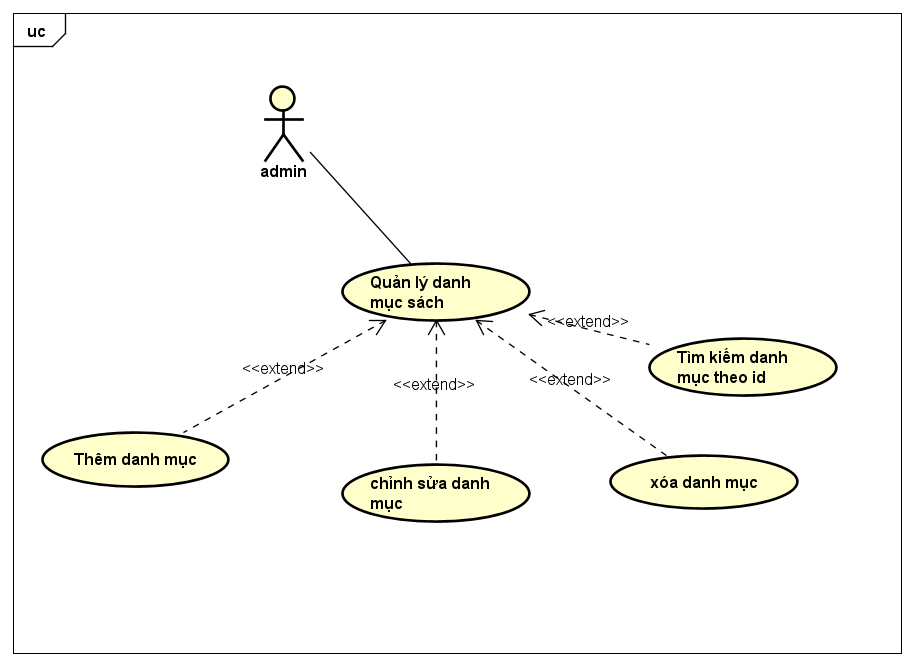
\includegraphics[width=1\linewidth]{Hinhve/quản lý danh mục sách.png}
\caption{Sơ đồ use case "Quản lý danh mục sách"}
\label{fig:UsecaseControlCategory}
\end{figure}
Với use case này cho phép admin đã có tài khoản có thể đăng nhập.Sau khi đăng nhập, admin có thể quản lý các danh mục của sách: thêm, sửa và xóa danh mục sách.

\subsection{Biểu đồ use case phân rã use case "Quản lý đơn hàng"}
\label{subsection:2.2.4}

\begin{figure}[H] % Chèn hình ảnh vào vị trí chính xác
\centering
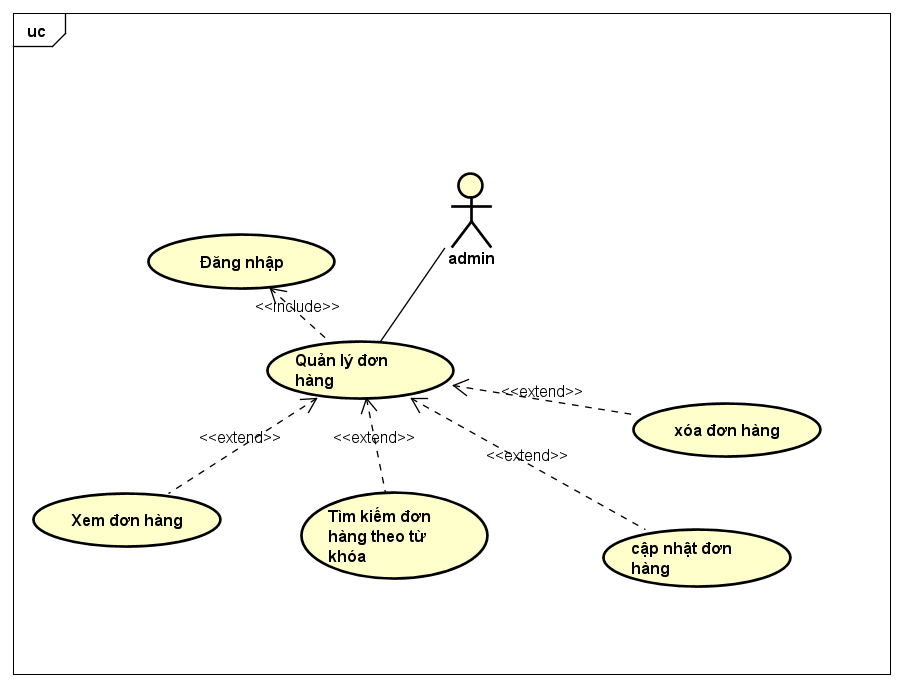
\includegraphics[width=1\linewidth]{Hinhve/quản lý đơn hàng.png}
\caption{Sơ đồ use case "Quản lý đơn hàng"}
\label{fig:UsecaseControlOrder}
\end{figure}
Với use case này cho phép admin đã có tài khoản có thể đăng nhập.Sau khi đăng nhập, admin có thể xem chi tiết từng đơn hàng, thêm, sửa thông tin hoặc xóa đơn hàng

\subsection{Biểu đồ use case phân rã use case "Quản lý sách"}
\label{subsection:2.2.7}

\begin{figure}[H] % Chèn hình ảnh vào vị trí chính xác
\centering
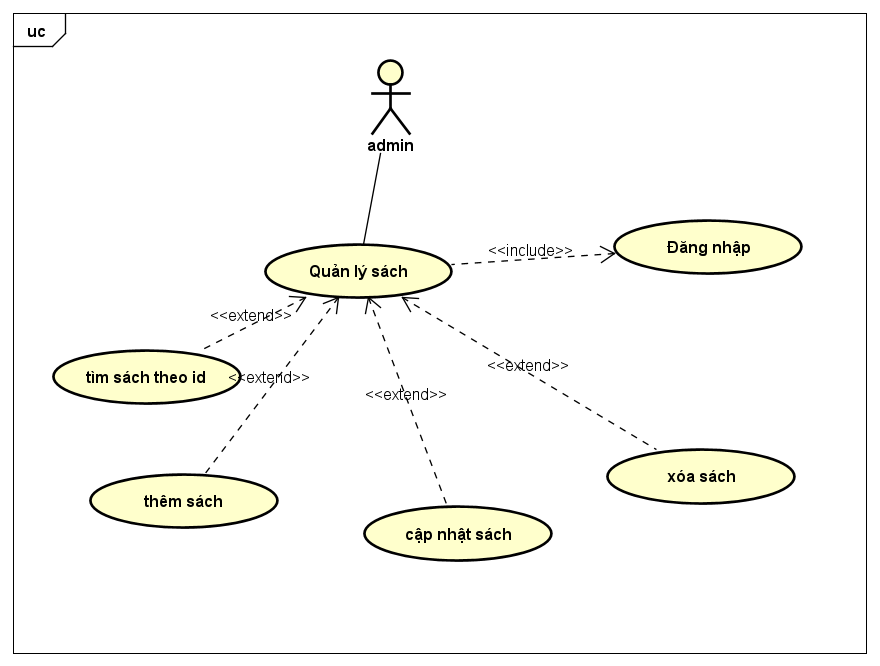
\includegraphics[width=1\linewidth]{Hinhve/quản lý sách.png}
\caption{Sơ đồ use case "Xem sách"}
\label{fig:UsecaseControlBook}
\end{figure}
Với use case này cho phép admin đã có tài khoản có thể đăng nhập.Sau khi đăng nhập, admin có thể xem chi tiết từng sách, thêm, sửa thông tin hoặc xóa sách.

\subsection{Biểu đồ use case phân rã use case "Xem sách"}
\label{subsection:2.2.6}

\begin{figure}[H] % Chèn hình ảnh vào vị trí chính xác
\centering
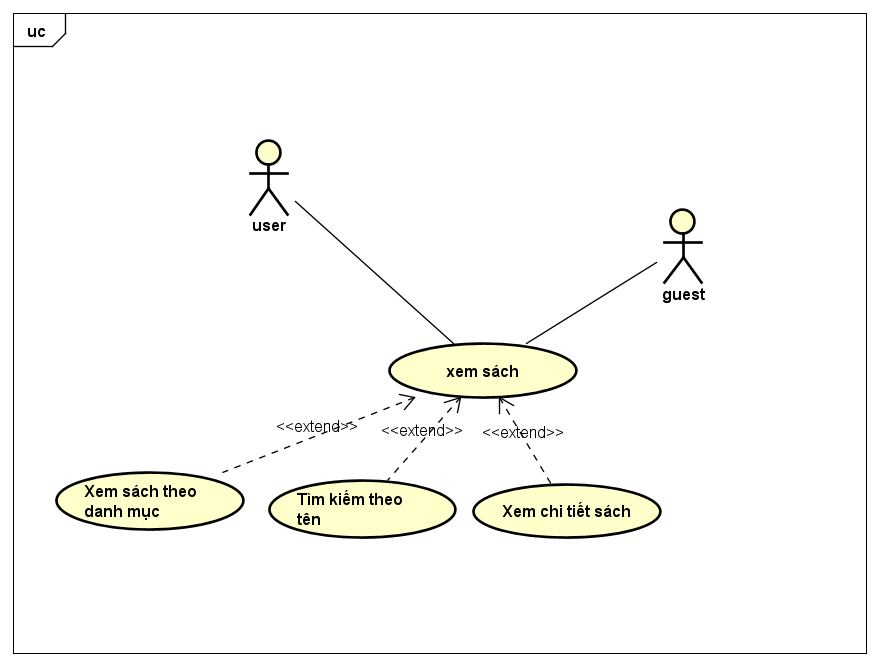
\includegraphics[width=1\linewidth]{Hinhve/xem sách.png}
\caption{Sơ đồ use case "Xem sách"}
\label{fig:UsecaseBook}
\end{figure}
Với use case này cho phép người dùng (user) hoặc khách(guest) có thể xem chi tiết từng sách, tìm kiếm sách theo tên, theo danh mục.


\subsection{Quy trình nghiệp vụ}
\label{subsection:2.2.7}
% Nếu sản phẩm/hệ thống cần xây dựng có quy trình nghiệp vụ quan trọng/đáng chú ý, sinh viên cần mô tả và vẽ biểu đồ hoạt động minh họa quy trình nghiệp vụ đó. Sinh viên lưu ý đây không phải là luồng sự kiện của từng use case, mà là luồng hoạt động kết hợp nhiều use case để thực hiện một nghiệp vụ nào đó.

% Ví dụ, một hệ thống quản lý thư viện có quy trình nghiệp vụ mượn trả với mô tả sơ bộ như sau: Sinh viên làm thẻ mượn, sau đó sinh viên đăng ký mượn sách, thủ thư cho mượn, và cuối cùng sinh viên trả lại sách cho thư viện. Một hệ thống có thể có một vài quy trình nghiệp vụ quan trọng như vậy.
\begin{figure}[H] % Chèn hình ảnh vào vị trí chính xác
\centering
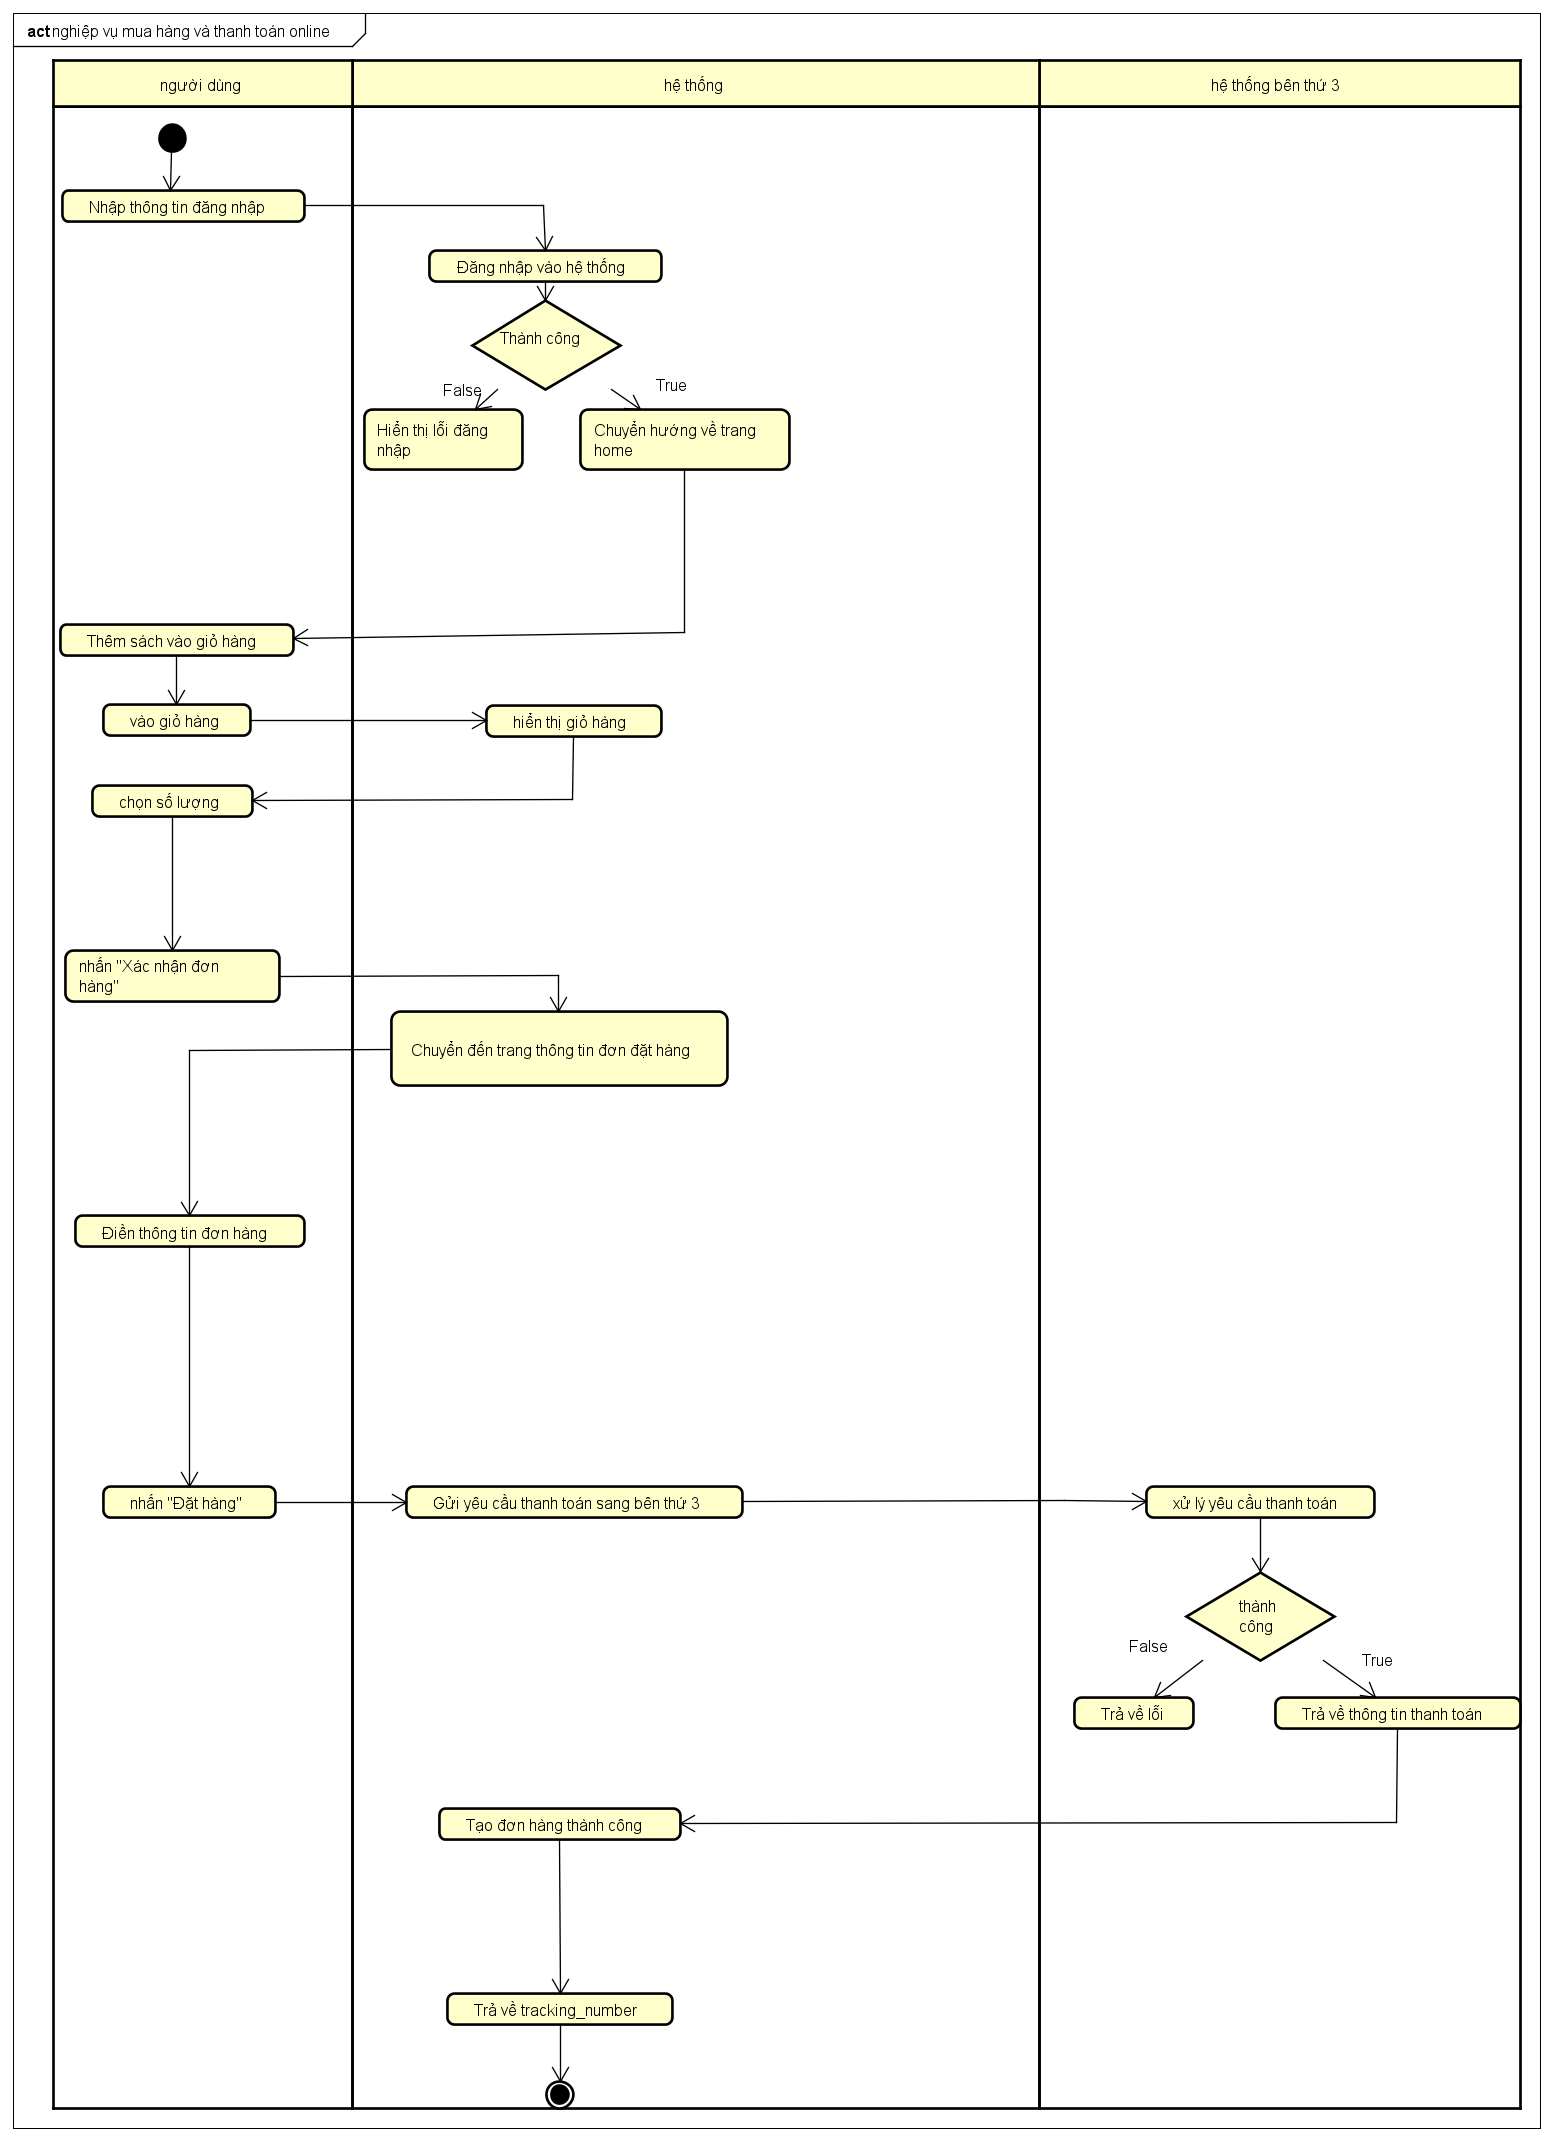
\includegraphics[width=1\linewidth]{Hinhve/nghiệp vụ mua hàng và thanh toán online.png}
\caption{Quy trình nghiệp vụ "đặt hàng và thanh toán trực tuyến"}
\label{fig:UsecaseBook}
\end{figure}

Người dùng đăng nhập bằng tài khoản đã đăng kí trong hệ thống. Sau khi đăng nhập, người dùng chọn sách mà mình muốn rồi cho vào giỏ hàng. Chuyển đến giỏ hàng, người dùng chọn số lượng cho từng sách. Sau khi chọn xong, người dùng sẽ chọn "Xác nhận đơn hàng". Hệ thống sẽ chuyển người dùng đến trang đặt hàng để người dùng có thể điền các thông tin cho đơn hàng. Sau khi điền xong, người dùng nhấn "Đặt hàng", hệ thống sẽ gửi yêu cầu thành toán cho bên thứ 3 đẻ xử lý thanh toán, khi xứ lý thành công, bên thứ 3 sẽ guwrri thông báo đến cho hệ thống và hệ thống sẽ tạo đơn hàng, trả về tracking number của đơn hàng cho người dùng.

\section{Đặc tả chức năng}
\label{section:2.3}

\subsection{Đặc tả use case "xem sách"}

\begin{NiceTabular}[width=\textwidth]{X[2,l]X[1,l]X[2,l]X[6,l]}[hvlines]
    \textbf{Mã usecase} & \Block[t,l]{1-3}{UC01} & & \\ 
    \textbf{Tên usecase} & \Block[t,l]{1-3}{Xem sách} & & \\ 
    \textbf{Tác nhân} & \Block[t,l]{1-3}{Người dùng, khách} & & \\ 
    \textbf{Mô tả} & \Block[t,l]{1-3}{Cho phép người dùng xem thông tin sách trên hệ thống bán sách \\trực tuyến} & & \\ 
    \textbf{Tiền điều kiện} & \Block[t,l]{1-3}{Không có} & & \\ 
    \Block{6-1}{\textbf{Luồng sự kiện chính}} & 
    \textbf{STT} & \textbf{Thực hiện bởi} & \textbf{Hành động} \\ 
    & 1 & Người dùng & Truy cập vào trang web \\ 
    & 2 & Người dùng & Chọn mục sách muốn xem \\ 
    & 3 & Hệ thống & Hiển thị danh sách sách \\ 
    & 4 & Người dùng & Ấn vào sách muốn xem \\ 
    & 5 & Hệ thống & Hiển thị thông tin chi tiết của sách \\ 
    \Block{2-1}{\textbf{Luồng sự kiện thay thế}} &   
    \textbf{STT} & \textbf{Thực hiện bởi} & \textbf{Hành động} \\ 
    &3a & Hệ thống & Nếu người dùng không chọn danh mục sách, hệ thống sẽ hiển thị tất cả các sách trong dữ liệu \\ 
    \textbf{Hậu điều kiện} & \Block[t,l]{1-3}{Người dùng có thể xem thông tin chi tiết của sách } & &
\end{NiceTabular}

\subsection{Đặc tả use case "Đăng nhập"}
\begin{NiceTabular}[width=\textwidth]{X[2,l]X[1,l]X[2,l]X[6,l]}[hvlines]
\textbf{Mã Usecase} & \Block[t,l]{1-3}{UC02} & & \\
\textbf{Tên Usecase} & \Block[t,l]{1-3}{Đăng nhập} & & \\
\textbf{Tác nhân} & \Block[t,l]{1-3}{Người dùng} & & \\
\textbf{Mô tả} & \Block[t,l]{1-3}{Cho phép người dùng đăng nhập vào hệ thống bán sách trực \\ tuyến} & & \\
\textbf{Tiền điều kiện} & \Block[t,l]{1-3}{Người dùng đã đăng ký tài khoản trên hệ thống} & & \\
\Block{8-1}{\textbf{Luồng sự kiện chính}} &
\textbf{STT} & \textbf{Thực hiện bởi} & \textbf{Hành động} \\
& 1 & Người dùng & Truy cập vào trang web \\
& 2 & Người dùng & Chọn "Đăng nhập" \\
& 3 & Hệ thống & Hiển thị form đăng nhập \\
& 4 & Người dùng & Nhập tên đăng nhập và mật khẩu \\
& 5 & Người dùng & Nhấn "Đăng nhập" \\
& 6 & Hệ thống & Kiểm tra thông tin đăng nhập \\
& 7 & Hệ thống & Nếu thông tin đúng, chuyển đến trang chủ \\
\Block{2-1}{\textbf{Luồng sự kiện thay thế}} &  
\textbf{STT} & \textbf{Thực hiện bởi} & \textbf{Hành động} \\
&5a & Hệ thống & Nếu thông tin sai, hiển thị thông báo lỗi và yêu cầu người dùng nhập lại hoặc chọn "Quên mật khẩu" \\
\textbf{Hậu điều kiện} & \Block[t,l]{1-3}{Người dùng được xác thực và có thể sử dụng các chức năng của \\ hệ thống} & &
\end{NiceTabular}


\subsection{Đặc tả use case "Đặt hàng trực tuyến"}

\begin{NiceTabular}[width=\textwidth]{X[2,l]X[1,l]X[2,l]X[6,l]}[hvlines]
\textbf{Mã Usecase} & \Block[t,l]{1-3}{UC03} & & \\
\textbf{Tên Usecase} & \Block[t,l]{1-3}{Đặt hàng trực tuyến} & & \\
\textbf{Tác nhân} & \Block[t,l]{1-3}{Người dùng} & & \\
\textbf{Mô tả} & \Block[t,l]{1-3}{Cho phép người dùng đặt mua sách trực tuyến từ hệ thống bán \\ sách} & & \\
\textbf{Tiền điều kiện} & \Block[t,l]{1-3}{Người dùng đã đăng nhập vào hệ thống} & & \\
\Block{11-1}{\textbf{Luồng sự kiện chính}} &
\textbf{STT} & \textbf{Thực hiện bởi} & \textbf{Hành động} \\
& 1 & Người dùng & Truy cập trang web và chọn sách muốn mua \\
& 2 & Người dùng & Thêm sách vào giỏ hàng \\
& 3 & Người dùng & Mở giỏ hàng \\
& 4 & Hệ thống & Hiển thị nội dung giỏ hàng \\
& 5 & Người dùng & Xác nhận đơn hàng \\
& 6 & Hệ thống & Hiển thị form nhập thông tin giao hàng và thanh toán \\
& 7 & Người dùng & Nhập thông tin giao hàng và thanh toán \\
& 8 & Người dùng & Nhấn "Đặt hàng" \\
& 9 & Hệ thống & Xác nhận thông tin và xử lý đơn hàng \\
& 10 & Hệ thống & Thông báo đặt hàng thành công \\
\Block{2-1}{\textbf{Luồng sự kiện thay thế}} &  
\textbf{STT} & \textbf{Thực hiện bởi} & \textbf{Hành động} \\
&6a & Hệ thống & Nếu thông tin nhập không hợp lệ, hiển thị thông báo lỗi và yêu cầu người dùng nhập lại thông tin \\
\textbf{Hậu điều kiện} & \Block[t,l]{1-3}{Đơn hàng được ghi nhận và xử lý, người dùng nhận được xác \\ nhận đặt hàng} & &
\end{NiceTabular}

\subsection{Đặc tả use case "Quản lý đơn hàng"}

\begin{NiceTabular}[width=\textwidth]{X[2,l]X[1,l]X[2,l]X[6,l]}[hvlines]
\textbf{Mã Usecase} & \Block[t,l]{1-3}{UC04} & & \\
\textbf{Tên Usecase} & \Block[t,l]{1-3}{Quản lý đơn hàng} & & \\
\textbf{Tác nhân} & \Block[t,l]{1-3}{Admin} & & \\
\textbf{Mô tả} & \Block[t,l]{1-3}{Quản lý các hoạt động liên quan đến đơn hàng trong hệ thống \\ bán sách trực tuyến từ khi đặt hàng đến khi giao hàng thành công\\ cho khách hàng.} & & \\
\textbf{Tiền điều kiện} & \Block[t,l]{1-3}{Admin đã đăng nhập vào hệ thống thành công, dữ liệu được truy\\ cập bình thường.} & & \\
\Block{7-1}{\textbf{Luồng sự kiện chính}} & 
\textbf{STT} & \textbf{Thực hiện bởi} & \textbf{Hành động} \\
& 1 & Admin & Truy cập trang quản trị và chọn "Đơn hàng" \\
& 2 & Hệ thống & Hiển thị danh sách các đơn hàng \\
& 3 & Admin & Chọn một đơn hàng cần thực hiện thao tác \\
& 4 & Hệ thống & Hiển thị chi tiết đơn hàng \\
& 5 & Admin & Thực hiện một trong các hành động sau:
    \begin{enumerate}
    \item[(i)] Xem chi tiết đơn hàng
    \item[(ii)] Sửa thông tin đơn hàng (thông tin khách hàng, địa chỉ giao hàng, trạng thái đơn hàng, ...)
    \item[(iii)] Xóa đơn hàng
    \end{enumerate} \\
& 6 & Hệ thống & Cập nhật và lưu lại các thay đổi khi Admin thực hiện các hành động sửa thông tin đơn hàng, xóa đơn hàng \\
\Block{3-1}{\textbf{Luồng sự kiện thay thế}} &  
\textbf{STT} & \textbf{Thực hiện bởi} & \textbf{Hành động} \\
&3a & Admin & Không thực hiện thao tác nào trên đơn hàng đã chọn \\
&3b & Hệ thống & Quay lại danh sách đơn hàng (bước 2) \\
\textbf{Hậu điều kiện} & \Block[t,l]{1-3}{Đơn hàng được cập nhật hoặc xóa thành công trong cơ sở dữ liệu} & &
\end{NiceTabular}

\subsection{Đặc tả use case "Quản lý sách"}
\begin{NiceTabular}[width=\textwidth]{X[2,l]X[1,l]X[2,l]X[6,l]}[hvlines]
\textbf{Mã Usecase} & \Block[t,l]{1-3}{UC05} & & \\
\textbf{Tên Usecase} & \Block[t,l]{1-3}{Quản lý sách} & & \\
\textbf{Tác nhân} & \Block[t,l]{1-3}{Admin} & & \\
\textbf{Mô tả} & \Block[t,l]{1-3}{Admin quản lý các hoạt động liên quan đến sách trong hệ thống\\ bán sách trực tuyến.} & & \\
\textbf{Tiền điều kiện} & \Block[t,l]{1-3}{Admin đã đăng nhập vào hệ thống thành công, dữ liệu sách có\\ sẵn.} & & \\
\Block{7-1}{\textbf{Luồng sự kiện chính}} & 
\textbf{STT} & \textbf{Thực hiện bởi} & \textbf{Hành động} \\
& 1 & Admin & Truy cập trang quản trị và chọn "Sách" \\
& 2 & Hệ thống & Hiển thị danh sách các sách hiện có trong cơ sở dữ liệu \\
& 3 & Admin & Chọn một sách cần thực hiện thao tác \\
& 4 & Hệ thống & Hiển thị chi tiết sách đã chọn \\
& 5 & Admin & Thực hiện một trong các hành động sau:
    \begin{enumerate}
    \item[(i)] Xem chi tiết sách
    \item[(ii)] Thêm sách mới
    \item[(iii)] Sửa thông tin sách (tên sách, tác giả, giá bán, ...)
    \item[(iv)] Xóa sách
    \end{enumerate} \\
& 6 & Hệ thống & Cập nhật và lưu lại các thay đổi khi Admin thực hiện các hành động sửa thông tin sách, thêm sách mới hoặc xóa sách \\
\Block{3-1}{\textbf{Luồng sự kiện thay thế}} &
\textbf{STT} & \textbf{Thực hiện bởi} & \textbf{Hành động} \\
&3a & Admin & Không thực hiện thao tác nào trên sách đã chọn \\
&3b & Hệ thống & Quay lại danh sách sách (bước 2) \\
\textbf{Hậu điều kiện} & \Block[t,l]{1-3}{Các thay đổi về sách được cập nhật thành công vào cơ sở dữ liệu\\ của hệ thống.} & &
\end{NiceTabular}


\subsection{Đặc tả usecase "Khiếu nại"}

\begin{NiceTabular}[width=\textwidth]{X[2,l]X[1,l]X[2,l]X[6,l]}[hvlines]
\textbf{Mã Usecase} & \Block[t,l]{1-3}{UC06} & & \\
\textbf{Tên Usecase} & \Block[t,l]{1-3}{Khiếu nại} & & \\
\textbf{Tác nhân} & \Block[t,l]{1-3}{Người dùng} & & \\
\textbf{Mô tả} & \Block[t,l]{1-3}{Người dùng khiếu nại về đơn hàng đã thực hiện trong hệ thống\\ bán sách trực tuyến.} & & \\
\textbf{Tiền điều kiện} & \Block[t,l]{1-3}{Người dùng đã đăng nhập vào hệ thống và đã xem được đơn hàng\\ của mình.} & & \\
\Block{8-1}{\textbf{Luồng sự kiện chính}} &
\textbf{STT} & \textbf{Thực hiện bởi} & \textbf{Hành động} \\
& 1 & Người dùng & Truy cập trang "Đơn hàng của tôi" \\
& 2 & Hệ thống & Hiển thị danh sách các đơn hàng của người dùng \\
& 3 & Người dùng & Chọn đơn hàng cần khiếu nại \\
& 4 & Hệ thống & Hiển thị form khiếu nại \\
& 5 & Người dùng & Nhập nội dung khiếu nại (lý do khiếu nại) \\
& 6 & Người dùng & Gửi khiếu nại \\
& 7 & Hệ thống & Ghi nhận khiếu nại, thông báo xử lý đến người dùng và chuyển đến bộ phận liên quan \\
\Block{2-1}{\textbf{Luồng sự kiện thay thế}} &
\textbf{STT} & \textbf{Thực hiện bởi} & \textbf{Hành động} \\
& \Block{1-3}{Không có} &  &  \\
\textbf{Hậu điều kiện} & \Block[t,l]{1-3}{Khiếu nại được gửi thành công và hệ thống ghi nhận để xử lý sau\\này. Người dùng có thể theo dõi trạng thái xử lý khiếu nại.} & &
\end{NiceTabular}


\subsection{Đặc tả use case "Thanh toán online"}
\begin{NiceTabular}[width=\textwidth]{X[2,l]X[1,l]X[2,l]X[6,l]}[hvlines]
\textbf{Mã Usecase} & \Block[t,l]{1-3}{UC07} & & \\
\textbf{Tên Usecase} & \Block[t,l]{1-3}{Thanh toán online} & & \\
\textbf{Tác nhân} & \Block[t,l]{1-3}{Người dùng, Hệ thống VNPAY} & & \\
\textbf{Mô tả} & \Block[t,l]{1-3}{Người dùng thực hiện thanh toán trực tuyến .} & & \\
\textbf{Tiền điều kiện} & \Block[t,l]{1-3}{Người dùng đã đăng nhập vào hệ thống và đã điền thôn tin giao\\ hàng và ấn "Đặt hàng"} & & \\
\Block{7-1}{\textbf{Luồng sự kiện chính}} &
\textbf{STT} & \textbf{Thực hiện bởi} & \textbf{Hành động} \\
& 1 & Hệ thống & Chuyển tới cổng thanh toán VNPAY \\
& 2 & Người dùng & Nhập các thông tin để thanh toán  \\
& 3 & Người dùng & Nhấn "Thanh toán" \\
& 4 & Hệ thống VNPAY & Gửi kết quả thanh toán (thành công hoặc thất bại) về hệ thống bán sách \\
& 5 & Hệ thống & Cập nhật trạng thái thanh toán của đơn hàng dựa trên kết quả nhận được từ VNPAY \\
& 6 & Hệ thống & Chuyển trở về trang chủ, xóa các sách trong giỏ hàng tạm thời \\
\Block{2-1}{\textbf{Luồng sự kiện thay thế}} &
\textbf{STT} & \textbf{Thực hiện bởi} & \textbf{Hành động} \\
& \Block{1-3}{Không có} &  & \\
\textbf{Hậu điều kiện} & \Block[t,l]{1-3}{Đơn hàng được thanh toán thành
công (nếu thanh toán thành\\ công) hoặc bị hủy (nếu thanh toán thất bại). Hệ thống cập nhật\\trạng thái thanh toán và ghi nhận thông tin thanh toán.} & &
\end{NiceTabular}

\section{Yêu cầu phi chức năng}
\label{section:2.4}
\subsection{Yêu cầu về bảo mật}
\label{subsection:2.4.1}
Hệ thống phải đảm bảo tính bảo mật vì có nhiều người sử dụng và các quyền hạn của từng người khác nhau. Do đó, hệ thống cần đảm bảo rằng người dùng chỉ có thể truy cập vào những tài nguyên mà họ được phép. 

Để bảo đảm an toàn cho người dùng và dữ liệu, hệ thống cung cấp các biện pháp bảo mật mạnh mẽ như sử dụng mã hóa dữ liệu đăng nhập của người dùng, xác thực, duy trì đăng nhập cho người dùng thông qua access token và cơ chế cấp lại token.
\subsection{Yêu cầu về thiết bị}
\label{subsection:2.4.2}
Hệ thống hiện đang phát triển dưới dạng web dành cho máy tính.

\subsection{Yêu cầu về giao diện người dùng}
\label{subsection:2.4.3}

Giao diện của hệ thống được thiết kế đơn giản nhưng tập trung vào các tính năng quan trọng, đồng thời mang đến cảm giác sử dụng thuận tiện cho người dùng. Giao diện của hệ thống được thiết kế để tương thích trên nhiều loại màn hình máy tính khác nhau.

\subsection{Yêu cầu về khả năng mở rộng}
\label{subsection:2.4.4}

Mục tiêu của hệ thống có thể kết nối với tất cả các loại thiết bị. Trong tương lai hệ thống chắc chắn cần những yêu cầu như vậy. Vì thế việc thiết kế hệ thống để dễ dàng nâng cấp và sửa đổi là vô cùng quan trọng. 

Hệ thống cần tương thích với nhiều nền tảng và giao thức khác nhau để có thể kết nối các thiết bị từ bên thứ ba. Điều này cho phép người dùng tích hợp các công nghệ khác nhau vào hệ thống.

\subsection{Yêu cầu về hiệu suất}
\label{subsection:2.4.4}

Hệ thống cần đạt các yêu cầu về hiệu suất bao gồm thời gian phản hồi nhanh, khả năng xử lý dữ liệu hiệu quả và nhanh chóng, cũng như khả năng xử lý tải lớn mà hiệu suất không kém đi.

\end{document}


%%%%%%%%%%%%%%%%%%%%%%%%%%%%%%%%%%%

\end{document}